% RL's Razor at 0.5B: write-up (setup and answers only). Every decimal number here is checked against
% figures/tables.md / tables.tex:
%   uv run python scripts/analyze.py --check-writeup writeup/writeup.tex --out figures/
% Build: cd writeup && pdflatex writeup.tex && pdflatex writeup.tex
\documentclass[11pt]{article}
\usepackage[margin=25mm]{geometry}
\usepackage[T1]{fontenc}
\usepackage[utf8]{inputenc}
\usepackage{lmodern}
\usepackage{booktabs,tabularx,graphicx,adjustbox,float,xcolor,enumitem,amsmath,amssymb}
\usepackage[skip=4pt]{caption}
\usepackage[hidelinks]{hyperref}
\hypersetup{pdftitle={RL's Razor at small scale: SFT vs GRPO forgetting on Qwen2.5-0.5B-Instruct and GSM8K},
  pdfauthor={Andrew Qiu}, pdfsubject={Reproduction of RL's Razor (Shenfeld, Pari, Agrawal, arXiv 2509.04259)}}
\graphicspath{{../figures/}}
\setlist{itemsep=1pt,topsep=2pt}
\emergencystretch=2em
\usepackage{xspace,needspace,xltabular}
\newcommand{\pp}{\,pp\xspace}
% reference keys (explained on page 1)
\newcommand{\T}[1]{\textsf{T:#1}}
\newcommand{\F}[1]{\textsf{F\S#1}}
\title{RL's Razor at small scale: SFT vs GRPO forgetting\\on Qwen2.5-0.5B-Instruct and GSM8K}
\author{Andrew Qiu\\[4pt]\normalsize Reproduction of \emph{RL's Razor} \cite{razor}}
\date{}

\begin{document}
\maketitle
\thispagestyle{empty}

\noindent\textbf{The task.} The take-home: reproduce RL's Razor's main result at small scale (Qwen2.5-0.5B-Instruct,
GSM8K, SFT vs GRPO, forgetting on unrelated benchmarks), then:
\begin{enumerate}[leftmargin=1.6em,itemsep=0pt]
\item Does SFT on the model's own correct answers forget like SFT or like RL?
\item Which method holds up better when you add noise to the labels or rewards?
\item How much general data do you need to mix into SFT before it forgets as little as RL?
\end{enumerate}
\noindent Section~\ref{sec:idea} summarises the paper's main idea and Section~\ref{sec:setup} our setup.
Section~\ref{sec:q0} is the main result (Q0) and Sections~\ref{sec:q1}--\ref{sec:q3} answer these three questions
(Q1--Q3); each opens with whether it was answered. Section~\ref{sec:why} explains why two of them are not fully
answered, and what would answer them. Limitations follow (Section~\ref{sec:limits}), and the last section,
Section~\ref{sec:proposal}, is a short proposal for Belvedir.
\texttt{README.md} gives the commands that reproduce every run, figure and table.

\medskip
{\small\noindent\textbf{How claims are referenced.} [1,~\S, p.] cites the paper by section and PDF page. Our results
cite a table, figure or section here and the \texttt{figures/tables.md} section holding the numbers: \T{Q0}--\T{Q3}
(those sections), \T{KL} (forward KL), \T{Bench} (per-benchmark change), \T{Data} (data and benchmark subsets),
\T{Cost} and \T{Div} (diverged runs). \F{n} is Section~n of \texttt{docs/paper-fidelity.md} (paper quotes, code
file:line); code paths are under \texttt{src/rlrazor/}. Assumptions are labelled as such.\par}

\medskip
\tableofcontents
\newpage

\section{The paper's main idea}
\label{sec:idea}
\textbf{Claim.} RL's Razor finds that ``even when SFT and RL achieve the same performance on the new task, \ldots\
SFT often achieves new-task gains by erasing prior knowledge, while RL better preserves old skills''
\cite[\S1, p.~2]{razor}, as the Pareto frontiers show \cite[\S3.1, pp.~4--5]{razor}.

\textbf{An empirical forgetting law.} The degree of forgetting ``is accurately predicted by
$\mathbb{E}_{x\sim\tau}\,\mathrm{KL}(\pi_0\|\pi)$, the KL divergence between the fine-tuned and base policy
evaluated on the new task'' \cite[\S1, p.~2]{razor}. A quadratic fit of forgetting on this KL gives $R^2 = 0.96$ in the
toy ParityMNIST setting and $0.71$ in the LLM experiments \cite[\S4, p.~6]{razor}. In ParityMNIST, SFT on an oracle,
KL-minimal label distribution forgets even less than RL \cite[\S4, p.~6]{razor}.

\textbf{Intuition.} On-policy RL samples outputs the model already finds likely and reweights them by reward, so it
moves to a nearby reweighted distribution; SFT pulls the model toward an external label distribution that can be
arbitrarily far away \cite[abstract, p.~1; \S5.2, p.~8]{razor}. The critical factor is on-policy data, not negative
gradients \cite[\S5.1, p.~8]{razor}.

\textbf{Theory.} For a finite output set, a convex policy family and a binary reward, and under regularity
conditions, policy gradient converges, among all optimal representable policies, to the one closest to the starting
policy in $\mathrm{KL}(\pi\|\pi_0)$ \cite[Theorem~5.2, \S5.2, p.~8]{razor}; the paper notes that neural-network
policy families may not converge exactly \cite[App.~A, p.~18]{razor}.

\textbf{The paper's caveats.} It lacks a mechanistic account of why larger KL shifts disrupt prior knowledge, its
behaviour at frontier scales is unknown, and it did not study off-policy algorithms \cite[\S7, pp.~9--10]{razor}.

\section{Setup}
\label{sec:setup}
We repeat at small scale the paper's LLM math experiment (Qwen2.5-3B-Instruct, SFT vs GRPO, models near each
method's Pareto frontier) \cite[\S3.1, p.~4; App.~B.1, p.~18]{razor}.

\textbf{Model, task and data.} Qwen2.5-0.5B-Instruct \cite{qwen25}; GSM8K \cite{gsm8k} (7,473 train / 1,319 test
prompts), Qwen chat template, final answer in \verb|\boxed{}| (\texttt{data/gsm8k.py}; \F{1}). Both methods draw on
the same train prompts; SFT keeps those with a correct teacher answer (\F{1}).

\textbf{Teacher SFT.} Targets are answers from Qwen2.5-7B-Instruct, sampled up to 16 times per prompt (7 distinct sampling seeds; \F{1}), keeping one
correct answer (98.1\% of prompts kept, 4.28 samples per prompt; \T{Data}). Cross-entropy on the answer tokens, AdamW,
constant LR with 50 warmup steps, batch 32, max grad norm 1, no weight decay, 2 epochs (epoch-1 and epoch-2
checkpoints; \texttt{train/sft.py}, \F{1}).

\textbf{GRPO.} Dr.~GRPO loss \cite{drgrpo} (no length normalisation, no per-group standard-deviation scaling of the
advantage), binary correctness reward, no KL penalty ($\beta = 0$), constant LR with 50 warmup steps; 1 epoch = 234
steps of 32 prompts $\times$ 8 completions, one gradient pass per batch, rollouts at temperature 1 with 512 new
tokens, checkpoints at steps 78, 156, 234 (\texttt{train/grpo.py}; \F{1}).

\textbf{Q1--Q3 arms} (\texttt{pipeline.py}, \texttt{data/}; \F{4}). The SFT-like arms use teacher SFT's settings, the
Q2 GRPO arm uses the GRPO settings, all at the best Q0 LRs (teacher SFT $3\times10^{-6}$, GRPO $10^{-6}$; Table~\ref{tab:headline}). \emph{Q1:} offline RFT samples 8
answers per prompt from the base model once and keeps one correct answer (81.5 to 82.1\% of prompts across seeds; \T{Data}); iterative RFT
runs 4 rounds, each sampling 4 answers per prompt from the current model, keeping one correct and training 1 epoch (warmup restarts each round);
self-rewrite SFT trains on the base model's rewrites of the reference solutions; SFT on GRPO outputs trains on
correct samples from the final checkpoint of GRPO seed 0 (1 seed). \emph{Q2:} SFT replaces a fraction
$p \in \{0.2, 0.4\}$ of its targets with another problem's teacher answer whose final answer differs from the true
one; GRPO flips each reward with probability $p$; 3 seeds each. \emph{Q3:} Tulu~3 \cite{tulu3} SFT rows are added
until they are a fraction $f \in \{0.02, 0.05, 0.1, 0.25, 0.5\}$ of the rows, 1 seed each, then 2 more seeds at
$f = 0.02$ and $0.05$.

\textbf{The forced LR deviation.} All three paper-range GRPO LRs ($10^{-5}$, $3\times10^{-5}$, $5\times10^{-5}$)
diverged at 0.5B: GSM8K $0.0$\% at the final checkpoint, outputs at the 512-token cap (\T{Div}; \F{3}). Teacher SFT
at every paper-range LR stayed at or below base (best $47.5$\% at $10^{-5}$) and forgot more as LR rose (\T{Q0}). We
therefore added GRPO at $10^{-6}$ and $3\times10^{-6}$, and teacher SFT and offline RFT at $3\times10^{-6}$. GRPO got
two low LRs and the SFT-like methods one (budget; \F{3}); this asymmetry favours GRPO. Diverged runs are excluded from
frontiers and from the KL fit (the pooled fit with them, over every evaluated checkpoint in \texttt{results/results.jsonl}, 127 including 13
from runs not reported here, is $R^2 = 0.38$; \T{Div}).

\textbf{Forgetting metric.} The paper's six prior-task benchmarks \cite[\S3.1, p.~4]{razor}: HellaSwag, TruthfulQA
(MC2), MMLU, IFEval \cite{ifeval}, Winogrande and HumanEval, through lm-eval \cite{lmeval} on vLLM in batch-invariant
(deterministic) mode (\texttt{eval/forgetting.py}, \texttt{eval/run\_eval.py}). To fit the budget, HellaSwag,
TruthfulQA and Winogrande are subsampled to 500 items each and MMLU to 10 per subject (570); IFEval and HumanEval are
complete (\T{Data}). Each benchmark has an item-sampling SE of $1.9$ to $3.7$\pp at the base score (\T{Data}). GSM8K is
scored greedily on all 1,319 test items (\texttt{eval/gsm8k.py}). Matched-accuracy comparisons follow the paper's
Pareto frontier with an exponential fit \cite[App.~B.1, p.~18]{razor}; the only target both methods reach is base
$+3$ = $51.1$\% (\T{Q0}).

\textbf{KL estimator.} Forward $\mathrm{KL}(\pi_0\|\pi)$ by Monte Carlo on 256 fixed GSM8K test prompts with one
cached base sample each (temperature 1, 512-token cap, EOS token not scored), scored in fp32; reported
in nats per sequence unless stated per token (\texttt{eval/kl.py}, \texttt{eval/run\_eval.py}; \F{1}). The paper
does not describe its estimator, so absolute values are not comparable to its plots (\F{1}).

\textbf{Seeds and compute.} 3 seeds at each method's best LR, 1 seed per sweep setting; the Q3 fractions
$f \ge 0.1$ and SFT on GRPO outputs are single runs (\T{Q0}, \T{Q3}). A seed changes the data order for every
method, and the rollouts for GRPO and the RFT arms; all teacher-SFT seeds share one teacher data set, the self-rewrite
seeds one greedy rewrite set, and the three offline-RFT seeds share six of their eight samples per prompt, so
SFT-side seed spreads leave out data-sampling variance (\texttt{pipeline.py}; \F{3}). Training ran on Modal A100-40GB GPUs and
evaluation on L4 GPUs, for a total Modal spend of \$83.11, which also covers smoke tests, pilots, diagnostics and runs not
reported here (Modal billing through the 22:00--23:00 UTC hour of 2026-11-22;
\T{Cost}).

\textbf{Deviations from the paper} that bear on the answers (all others, with verbatim quotes: \F{2}--\F{4}):
\begin{itemize}
\item 0.5B instead of 3B; GSM8K, not Open-Reasoner-Zero math; math only (assignment; \F{3}).
\item Teacher Qwen2.5-7B-Instruct instead of DeepSeek R1 for SFT targets (budget; \F{3}).
\item LRs below the paper's range for both methods (forced, above); three LRs per method in the paper-range sweep, not
  five, and one SFT scheduler and batch size (budget; \F{3}).
\item Group shape 32 prompts $\times$ 8 completions; under a literal reading of the paper's ``Group Size 64''
  \cite[Table~2, p.~19]{razor} our group is 8$\times$ smaller (budget; \F{3}). Advantages are not divided by the
  group standard deviation (Dr.~GRPO; \F{1}).
\item Frontier points are saved checkpoints (3 per GRPO run, 2 per SFT-like run, 4 per iterative-RFT run, one per round) plus the base model, not only final
  models of distinct configurations (budget; \F{3}).
\item Benchmark subsets and KL estimator above (budget; the paper gives no estimator; \F{3}).
\item Q3's general rows carried the GSM8K system prompt (R56 in \texttt{docs/rulings.md}; \F{4}).
\item fp32 master weights and bf16 autocast, so small RL updates are not rounded away (R13; \F{1}).
\end{itemize}

\section{Q0 baseline: SFT vs GRPO, and does KL predict forgetting?}
\label{sec:q0}
\textbf{Main result (Q0): partly reproduced.} Same sign at matched accuracy: at the shared $51.1$\% target SFT is
$0.1$ to $0.6$\pp worse than GRPO, within noise (final checkpoints: GRPO $0.25 \pm 0.16$, SFT $-0.05 \pm 0.19$\pp,
$p = 0.110$; GRPO learns more, $55.1$ vs $51.2$\% GSM8K, base $48.1$\%; Table~\ref{tab:headline}, \T{Q0}). The
IFEval split, post hoc: SFT $-3.5 \pm 1.2$ vs GRPO $+1.4 \pm 0.5$\pp ($p = 0.010$ uncorrected, $0.057$ after Bonferroni; \T{Bench}). Forward-KL $R^2$ is
$0.30$ (Figure~\ref{fig:kl}, \T{KL}) vs the paper's $0.71$ \cite[\S4, p.~6]{razor}. Values are mean $\pm$ seed
standard deviation over 3 seeds at each method's best LR, final checkpoints, unless marked; ``forgetting'' is the
mean change over the six benchmarks, checkpoint $-$ base, in pp (negative means forgetting).

\begin{table}[!htb]
\centering\small
\caption{Final checkpoints at each method's best setting (mean $\pm$ seed std). Forgetting in pp, checkpoint $-$
base; Welch test of forgetting vs GRPO. Q0 is the first two rows; the rest are the Q1 arms. Source: \T{Q0}.}
\label{tab:headline}
\begin{adjustbox}{max width=\linewidth}
\begin{tabular}{lrrrrr}
\toprule
Best setting & Seeds & GSM8K (\%) & Forgetting (pp) & KL (nats/seq) & $p$ vs GRPO\\
\midrule
GRPO, LR $10^{-6}$ & 3 & $55.1 \pm 1.4$ & $0.25 \pm 0.16$ & 50.52 & --\\
Teacher SFT, LR $3\times10^{-6}$ & 3 & $51.2 \pm 0.4$ & $-0.05 \pm 0.19$ & 10.43 & 0.110\\
\midrule
Offline RFT, LR $3\times10^{-6}$ & 3 & $49.4 \pm 0.5$ & $0.55 \pm 0.33$ & 5.54 & 0.257\\
Iterative RFT, LR $3\times10^{-6}$ & 3 & $51.4 \pm 2.2$ & $0.32 \pm 0.53$ & 9.54 & 0.828\\
Self-rewrite SFT, $3\times10^{-6}$ & 3 & $47.0 \pm 0.8$ & $-0.48 \pm 0.13$ & 37.94 & 0.004\\
SFT on GRPO outputs, $3\times10^{-6}$ & 1 & 51.6 & 0.13 & 50.57 & --\\
\bottomrule
\end{tabular}
\end{adjustbox}
\end{table}

\textbf{Accuracy and forgetting.} GRPO gains $7.1$ GSM8K points over base, teacher SFT $3.1$ (\T{Q0}). Mean
forgetting differs by $0.30$\pp (Welch $t = -2.06$, $p = 0.110$, $n = 3+3$; \T{Q0}): no measurable difference, and
neither forgets in the mean. At the shared $51.1$\% target, SFT $-$ GRPO is between $-0.1$ and $-0.6$\pp depending on
the reading (pooled fit, interpolation, or seed bands: GRPO $0.0 \pm 0.1$\pp on 3/3 seeds, SFT $-0.1$\pp on 2/3;
\T{Q0}): the paper's sign, within noise. The target lies below GRPO's lowest frontier point ($52.4$\%), so GRPO's
pooled value there is one point held downward (\T{Q0}), and GRPO contributes 12 low-LR checkpoints to SFT's 6
(Section~\ref{sec:setup}), which favours GRPO.

\textbf{IFEval (post hoc).} The mean hides one consistent difference: teacher SFT loses $3.5 \pm 1.2$\pp on IFEval (all
three seeds negative) while GRPO gains $1.4 \pm 0.5$\pp, Welch $p = 0.010$ uncorrected, $0.057$ after a Bonferroni
correction over the six benchmarks (\T{Bench}). SFT's mean is pulled back to zero by Winogrande ($1.6 \pm 0.3$) and
HumanEval ($1.4 \pm 0.7$; \T{Bench}).

\textbf{The clear forgetting is an LR effect.} Teacher SFT at three of the paper's LRs forgets more as the LR rises: $-0.5$,
$-4.9$, $-12.2$\pp at $10^{-5}$, $3\times10^{-5}$, $7\times10^{-5}$ (GSM8K $47.5$, $38.4$, $27.3$\%; 1 seed each;
\T{Q0}). GRPO at its paper-range LRs ($10^{-5}$, $3\times10^{-5}$, $5\times10^{-5}$) diverged instead (\T{Div}).

\begin{figure}[!htb]
\centering
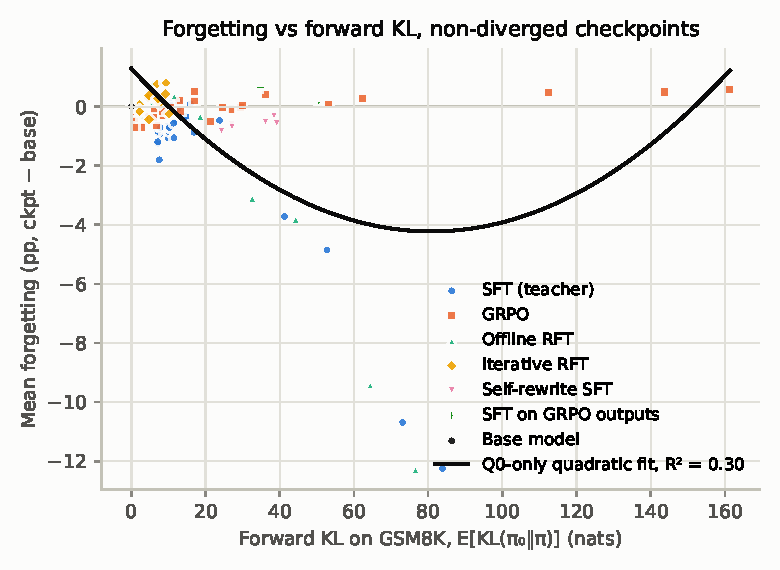
\includegraphics[width=\dimexpr\linewidth*3/5]{kl_vs_forgetting.pdf}
\caption{Forgetting vs forward KL, all non-diverged checkpoints of the Q0--Q3 arms, with the Q0-only quadratic fit.
Source: \T{KL}.}
\label{fig:kl}
\end{figure}

\textbf{Forward KL does not predict forgetting across methods.} The Q0-only quadratic fit of mean forgetting on KL
(teacher SFT, GRPO and base, 25 checkpoints) gives $R^2 = 0.30$ (\T{KL}), against the paper's $0.71$, which covers
SFT and RL models only \cite[\S4, p.~6; Fig.~11, p.~23]{razor}; per-token or median KL give $0.30$ and $0.29$ (\T{KL}). Within
SFT-like runs $R^2 = 0.91$, but that is the LR dose--response: restricted to LR $\le 3\times10^{-6}$ it falls to
$0.17$ (\T{KL}). \emph{Ordering caveat:} at the final checkpoints GRPO's KL is $50.52$ nats per sequence vs teacher
SFT's $10.43$, with no more forgetting (Table~\ref{tab:headline}), the opposite of the paper's ordering
\cite[\S4, p.~5; \S5.1, p.~8]{razor}. This is not driven by outliers or length (per-token ordering is the same),
and each method drifts on different samples (cross-method Spearman $0.22$; \T{KL}). It is consistent with GRPO
sharpening its policy (rollout entropy falls from $0.322$ to $0.127$ nats/token on seed 0; \T{KL}), but that link is
untested and SFT's rollout entropy was not logged. At near-equal accuracy the KL order flips: within 1 point of
$51.1$\%, GRPO has KL $6.46$ vs SFT's $9.67$, the paper's direction, but on only 2 GRPO checkpoints, which
forget slightly more ($-0.36$ vs $-0.09$\pp; \T{KL}). In neither case does KL track forgetting across methods.


\needspace{7\baselineskip}
\section{Q1: SFT on the model's own correct answers}
\label{sec:q1}
\textbf{Answered on the mean: like RL, but weakly; on IFEval (post hoc), iterative RFT forgets like SFT.} Offline and
iterative RFT $\approx$ GRPO on the six-benchmark mean (iterative $0.32 \pm 0.53$\pp, $p = 0.828$; offline
$0.55 \pm 0.33$\pp, $p = 0.257$; Table~\ref{tab:headline}), but the mean does not separate teacher SFT from GRPO
($p = 0.110$), so ``like RL'' is weak: teacher SFT barely forgot. On IFEval, the one benchmark that
separated them (post hoc; $p = 0.010$ uncorrected, $0.057$ after Bonferroni), iterative RFT loses $2.6 \pm 0.3$\pp, like teacher SFT (\T{Bench}); offline RFT
barely learns ($49.4$\%).

\begin{figure}[t]
\centering
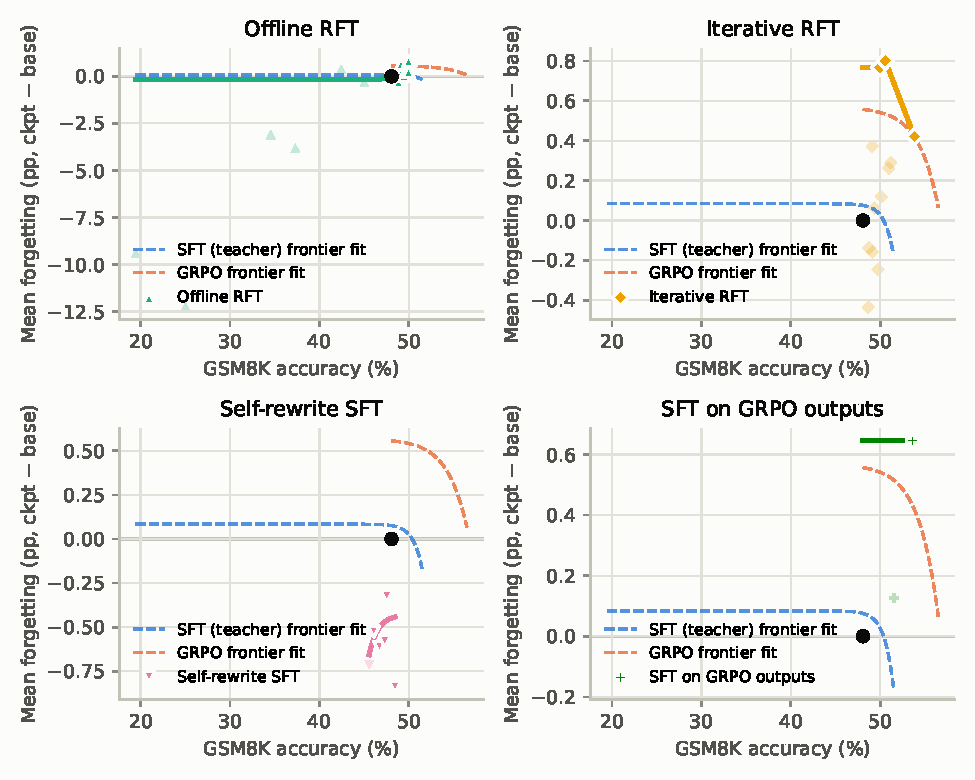
\includegraphics[width=\linewidth]{q1_selfgen.pdf}
\caption{Q1 arms, all checkpoints (faint) and frontier (solid), against the teacher-SFT and GRPO frontier fits
(dashed); black dot = base model. Seed means are in Table~\ref{tab:headline}. Source: \T{Q1}.}
\label{fig:q1}
\end{figure}

\textbf{Evidence} (Table~\ref{tab:headline}, lower rows; Figure~\ref{fig:q1}). Iterative RFT ends at
$51.4 \pm 2.2$\% GSM8K with $0.32 \pm 0.53$\pp mean forgetting, indistinguishable from GRPO ($p = 0.828$); at the
$51.1$\% target 2 of 3 seeds reach it with $0.5$\pp (\T{Q1}). On IFEval (post hoc, as in Q0), the one benchmark that separated SFT
from GRPO ($p = 0.010$ uncorrected, $0.057$ after Bonferroni), it loses $2.6 \pm 0.3$\pp on every seed, like teacher SFT ($-3.5 \pm 1.2$) and unlike GRPO ($1.4 \pm 0.5$;
Welch $p = 0.003$ after Bonferroni over the six benchmarks; \T{Bench}). Its mean is held up by HumanEval
($3.9 \pm 2.5$\pp) and Winogrande ($1.7 \pm 0.6$; \T{Bench}). At the paper's LRs, self-generated data forgets like
teacher data at the same LR (offline RFT $-0.3$, $-3.8$, $-12.3$\pp vs teacher SFT $-0.5$, $-4.9$, $-12.2$\pp; 1 seed
each; \T{Q1}, \T{Q0}): the LR, not the data's origin, governs forgetting there.

\needspace{4\baselineskip}\textbf{Caveats.}
\begin{itemize}
\item Offline RFT at $3\times10^{-6}$ barely learns ($49.4 \pm 0.5$\%, KL $5.54$); its forgetting ($0.55 \pm 0.33$\pp,
  $p = 0.257$) cannot be compared with GRPO's at a $1.3$-point gain (Table~\ref{tab:headline}).
\item SFT on GRPO outputs is 1 seed ($51.6$\%, $0.13$\pp). It drifts on the same samples as its source (Spearman
  $0.88$) but ends with more KL than that source ($50.57$ vs $36.05$) at lower accuracy ($51.6$ vs $53.8$\%; \T{KL}).
  Consistent with the paper's ParityMNIST distillation result (SFT on an RL model's outputs matches its
  trade-off; \cite[\S4, p.~6; Fig.~9, p.~22]{razor}); it does not establish it at this scale.
\item Self-rewrite SFT ends below base ($47.0 \pm 0.8$\%, $-0.48 \pm 0.13$\pp, $p = 0.004$ vs GRPO), but about 28\%
  of its rows fall back to gold text (\T{Data}), so no conclusion about wording is drawn.
\end{itemize}

\section{Q2: label noise (SFT) vs reward noise (GRPO)}
\label{sec:q2}
\textbf{Half answered.} \emph{Forgetting: answered.} Noise causes no measurable forgetting for either method (all
within $\pm 0.5$\pp; Table~\ref{tab:q2}). The finding is weak: neither method forgets much even without noise, so it
cannot show which would hold up better where SFT does forget (Section~\ref{sec:why}). \emph{Accuracy: mixed.} GRPO is
ahead at $p = 0$ and $0.2$ but loses more to noise ($-2.9$ vs $-1.7$\pp at $p = 0.2$; $-7.2$ vs $-4.7$\pp at
$p = 0.4$); the $p = 0.4$ gap is unresolved ($p = 0.309$; Table~\ref{tab:q2}). The data do not show that a noisy
outcome is safer as a reward than as a label.

\begin{table}[!htb]
\centering\small
\caption{Q2, final checkpoints, 3 seeds per cell (mean $\pm$ seed std). $p = 0$ is the Q0 best setting. Gap:
GRPO $-$ teacher SFT GSM8K, Welch test over seeds. Source: \T{Q2}.}
\label{tab:q2}
\begin{adjustbox}{max width=\linewidth}
\begin{tabular}{lrrrrrr}
\toprule
Arm & $p$ & GSM8K (\%) & Forgetting (pp) & IFEval (pp) & KL (nats/seq) & GSM8K gap (pp), $p$-value\\
\midrule
Teacher SFT & 0 & $51.2 \pm 0.4$ & $-0.05 \pm 0.19$ & $-3.5 \pm 1.2$ & 10.43 & \\
Teacher SFT & 0.2 & $49.5 \pm 0.6$ & $-0.04 \pm 0.20$ & $-2.3 \pm 1.2$ & 12.92 & \\
Teacher SFT & 0.4 & $46.5 \pm 1.3$ & $-0.23 \pm 0.29$ & $-2.5 \pm 0.4$ & 15.16 & \\
GRPO & 0 & $55.1 \pm 1.4$ & $0.25 \pm 0.16$ & $1.4 \pm 0.5$ & 50.52 & $4.0$, $0.029$\\
GRPO & 0.2 & $52.2 \pm 1.2$ & $-0.11 \pm 0.35$ & $0.2 \pm 0.9$ & 20.90 & $2.7$, $0.040$\\
GRPO & 0.4 & $48.0 \pm 1.8$ & $0.06 \pm 0.41$ & $0.2 \pm 0.8$ & 11.93 & $1.5$, $0.309$\\
\bottomrule
\end{tabular}
\end{adjustbox}
\end{table}

\textbf{Evidence} (Table~\ref{tab:q2}, \T{Q2}). Change in GSM8K from $p = 0$: teacher SFT $-1.7$ and $-4.7$\pp, GRPO
$-2.9$ and $-7.2$\pp at $p = 0.2$ and $0.4$, so GRPO loses more accuracy to noise at both rates. It is still ahead at
$p = 0.2$ (Welch $t = 3.60$) because its clean lead ($4.0$\pp) only shrinks. All six mean-forgetting values lie inside
$\pm 0.5$\pp, with seed std up to $0.41$\pp. Corrupted labels do not make SFT forget more; its IFEval loss stays at
about $-2.5$\pp, and GRPO's IFEval gain shrinks to $0.2$\pp.

\needspace{4\baselineskip}\textbf{Caveats.}
\begin{itemize}
\item The data do not show that a noisy outcome is safer used as a reward than as a label: GRPO's drops ($-2.9$,
  $-7.2$\pp) are larger than SFT's ($-1.7$, $-4.7$\pp; \T{Q2}).
\item At $p = 0.4$ the gap ($48.0 \pm 1.8$ vs $46.5 \pm 1.3$\%, $t = 1.19$, $p = 0.309$; \T{Q2}) is not resolved, and
  both arms are back near base accuracy, so neither method is shown to be more robust at the higher rate.
\item The two corruptions differ (wrong targets vs flipped rewards; Section~\ref{sec:setup}), so this compares
  practical robustness, not equal information loss. The realised number of corrupted rows was not recorded in
  \texttt{results/} (\F{4}).
\end{itemize}

\section{Q3: mixing general instruction data into SFT}
\label{sec:q3}
\textbf{Not answered in this setup.} Plain SFT misses the threshold by only $0.014$\pp (inside the GRPO band's sd of
$0.10$\pp; \T{Q3}), so there was no gap for mixing to close. The pre-registered IFEval criterion fails at every $f$
(Table~\ref{tab:q3}), and that result carries a confound: the general (Tulu~3) rows were trained under a system prompt
that asks for a \texttt{\textbackslash boxed\{\}} answer (\F{4}).

\textbf{In detail.} The data do not give a fraction. The pre-registered primary criterion, the smallest $f$ whose mean
forgetting at GRPO's matched target ($51.1$\%) is at least GRPO's mean $-$ 1 sd there, does not discriminate, and the
secondary criterion (the same rule on IFEval) fails at every $f$, under a confound (\T{Q3}; R54 in
\texttt{docs/rulings.md}).

\begin{table}[!htb]
\centering\small
\caption{Q3: teacher SFT at $3\times10^{-6}$ with a fraction $f$ of Tulu~3 rows. Forgetting at $51.1$\% GSM8K uses
only the seeds that reach it. Final columns: mean $\pm$ seed std. GRPO: forgetting $0.0 \pm 0.1$ and IFEval
$0.7 \pm 0.9$\pp at the target, final IFEval $1.4 \pm 0.5$\pp. Source: \T{Q3}.}
\label{tab:q3}
\begin{adjustbox}{max width=\linewidth}
\begin{tabular}{lrrrrrr}
\toprule
$f$ & Seeds & At $51.1$\%: forgetting (pp) & At $51.1$\%: IFEval (pp) & Final GSM8K (\%) & Final forgetting (pp)
& Final IFEval (pp)\\
\midrule
0 & 3 & $-0.109$ (2/3) & $-3.2$ (2/3) & $51.2 \pm 0.4$ & $-0.05 \pm 0.19$ & $-3.5 \pm 1.2$\\
0.02 & 3 & $-0.187$ (1/3) & $-4.3$ (1/3) & $50.9 \pm 1.1$ & $-0.29 \pm 0.45$ & $-5.5 \pm 1.2$\\
0.05 & 3 & $-0.290$ (2/3) & $-5.5$ (2/3) & $52.0 \pm 1.1$ & $-0.07 \pm 0.10$ & $-7.0 \pm 0.7$\\
0.1 & 1 & $-1.236$ & $-8.7$ & 50.8 & $-1.06$ & $-8.1$\\
0.25 & 1 & not reached & not reached & 49.4 & $-0.83$ & $-7.4$\\
0.5 & 1 & $-0.771$ & $-7.9$ & 50.7 & $-0.67$ & $-7.8$\\
\bottomrule
\end{tabular}
\end{adjustbox}
\end{table}

\textbf{Evidence, primary criterion} (\T{Q3}). The threshold is $0.005 - 0.100 = -0.095$\pp. Unmixed SFT ($f = 0$)
misses it by $0.014$\pp on the mean of the 2 of 3 seeds that reach the target ($-0.196$ and $-0.022$; the third tops out at $50.7$\%), inside the GRPO
band's sd of $0.10$\pp and far below the item SE of any benchmark (\T{Data}). The mixed runs miss it too ($f = 0.05$:
seeds $0.030$ and $-0.610$), so the rule as coded returns no crossover for $f \le 0.5$. What the data support is
narrower: no seeded $f$ ($\le 0.05$) is distinguishable from GRPO, or from unmixed SFT, on mean forgetting, and the
criterion cannot rank the mixes. Mixing never lifts final GSM8K into GRPO's range (below $53.8$\%, GRPO's mean $-$ sd,
at every $f$).

\textbf{Evidence, IFEval criterion (pre-registered): fails at every $f$} (Table~\ref{tab:q3}, \T{Q3}). At the target
IFEval is $-3.2$ to $-8.7$\pp against a threshold of $-0.3$\pp. On final checkpoints IFEval worsens as $f$ grows from
0 to $0.05$: $-3.5 \pm 1.2$, $-5.5 \pm 1.2$, $-7.0 \pm 0.7$\pp; the $0 \to 0.02$ step alone is not resolved by 3 seeds
(Welch $p = 0.097$, uncorrected), the $0 \to 0.05$ step is ($p = 0.017$).

\textbf{Confound, stated next to the result.} Every training row, including the Tulu~3 rows, was formatted with the
GSM8K system prompt, which asks for the final answer in \verb|\boxed{}|; the Tulu responses do not give one (\F{4}).
Training the model to ignore that instruction on 2 to 50\% of rows may by itself lower an instruction-following
benchmark (assumption, untested). We therefore do \emph{not} read the IFEval result as support for the paper's
``off-policy data forgets'' account, nor as evidence that general-data replay hurts in general; it is a result about
this mixing recipe.

\needspace{4\baselineskip}\textbf{Further caveats.}
\begin{itemize}
\item The fractions $f \ge 0.1$ are single-seed. They are lower ($-0.8$ and $-1.2$\pp at the target; final $-0.67$ to
  $-1.06$\pp) but cannot be tested with one seed, and their mean is dominated by IFEval: its drop ($-7.4$ to
  $-8.1$\pp), entering the six-benchmark mean with weight one sixth, is larger than the whole mean drop
  (Table~\ref{tab:q3}).
\item Seeds were added only at $f = 0.02$ and $0.05$, the bracket of the 1-seed crossover (\F{4}). The realised number
  of added rows was not recorded in \texttt{results/}; the step counts match the intended mix sizes (\F{4}).
\end{itemize}

\section{Why two of the three questions are not fully answered, and what would answer them}
\label{sec:why}
\textbf{It was not a budget choice.} The three GRPO learning rates we ran from the paper's range ($10^{-5}$,
$3\times10^{-5}$, $5\times10^{-5}$, of the five in \cite[Table~2, p.~19]{razor}) all diverged at 0.5B. At $10^{-5}$,
GSM8K fell to $0.0$\% by step 156 and stayed there at step 234 (\T{Div}), with 512-token completions (greedy
diagnostic in \T{KL}; \F{3}). Teacher SFT at the paper's $10^{-5}$ and $3\times10^{-5}$ ended at or below base accuracy
($47.5$\% and $38.4$\% vs $48.1$\%; \T{Q0}), so there is no matched-accuracy point to compare. Hence the forced lower
rates (R47 and R50 in \texttt{docs/rulings.md}).

\textbf{At the rates that did train, there is little forgetting to measure against.} At GRPO $10^{-6}$ and SFT
$3\times10^{-6}$, SFT barely forgets on the six-benchmark mean ($-0.05 \pm 0.19$\pp; Table~\ref{tab:headline}). That
shrinks the SFT--RL gap that Q1--Q3 measure against to about seed noise ($0.30$\pp, $p = 0.110$; \T{Q0}). That is why
Q2's forgetting result, though answered, is weak and Q3 cannot separate the methods: neither noise nor mixing can
visibly change a gap that 3 seeds do not resolve from seed noise to begin with (Sections~\ref{sec:q2}, \ref{sec:q3}). The same limit is
why Q1's contrast is small. The open half of Q2 is accuracy, and it is open for a different reason: GRPO is ahead at
$p = 0$ and $p = 0.2$ but loses more to noise, and at $p = 0.4$ three seeds do not resolve the gap
(Table~\ref{tab:q2}).

\textbf{Where SFT does forget, it does not learn.} Mean SFT forgetting appears only at high LR ($-0.5$, $-4.9$,
$-12.2$\pp at $10^{-5}$, $3\times10^{-5}$, $7\times10^{-5}$; 1 seed each), and there it comes without a GSM8K gain
($47.5$, $38.4$, $27.3$\% against base $48.1$\%; \T{Q0}).

\textbf{What would answer them.} Rerun on the paper's own model, Qwen2.5-3B-Instruct, at the paper's Table~2 learning
rates \cite[\S3.1, p.~4; Table~2, p.~19]{razor}. A small pilot comes first, one GRPO run and one SFT run, to confirm
that GRPO trains stably there and that SFT forgets measurably while gaining accuracy; only then would the Q2 noise
arms and Q3 mixing fractions be rerun against a real SFT--RL gap. This is an expectation (an assumption), not a
result: nothing was run at 3B.

\section{Limitations}
\label{sec:limits}
\begin{itemize}
\item \textbf{One small model, one task, low LRs.} 0.5B and GSM8K only, at LRs below the paper's range (one for SFT,
  two for GRPO; Section~\ref{sec:setup}). SFT's forgetting appears here only at LRs where
  SFT also loses GSM8K (\T{Q0}), and Q2 and Q3 inherit little mean forgetting to change (Section~\ref{sec:why}).
\item \textbf{One shared target.} $51.1$\% is below GRPO's frontier; only 2 of 3 SFT seeds reach it (\T{Q0}).
\item \textbf{Power.} 3 seeds; item SE $1.9$ to $3.7$\pp per benchmark (\T{Data}). IFEval is post hoc in Q0
  (pre-registered only as Q3's secondary criterion; R54). Mean-forgetting effects in Q2 and the seeded Q3 fractions
  are inside $\pm 0.5$\pp; the exception is a set of single runs, Q3 at $f \ge 0.1$ (final $-0.67$ to $-1.06$\pp,
  driven by the IFEval drop; Tables~\ref{tab:q2} and~\ref{tab:q3}). Single runs: Q3 at $f \ge 0.1$, SFT on GRPO
  outputs. lm-eval kept only aggregate scores (\texttt{eval/forgetting.py}), so a paired item-level bootstrap would
  need re-evaluation on GPU.
\item \textbf{Confounds.} Q3's system prompt on general rows (\F{4}); self-rewrite's gold fallback (about 28\% of
  rows; \T{Data}).
\item \textbf{KL estimator.} 256 prompts, one temperature-1 base sample each, 512-token cap, EOS not scored
  (\texttt{eval/kl.py}; \F{1}).
\end{itemize}

\section{Proposal for Belvedir}
\label{sec:proposal}
\textbf{Current workflow} (Belvedir's public website and job descriptions \cite{belvedir}). Four steps:
collect, train, evaluate, and deploy ``at scale'' while continuing ``training as new data arrives''. In detail:
pipelines for ``collection, cleaning, filtering, and synthesis'' of raw customer data;
training by ``SFT, distillation, preference tuning, and RL'', with asynchronous RL; ``task-specific evaluations''
that ``drive decisions about data and training recipes'', and benchmark creation; and a serving stack on Kubernetes
with ``batching, caching, routing, and autoscaling''. Since training continues, every lap is another fine-tune (my inference).
Neither model promotion nor multi-tenancy is described publicly.

\textbf{The proposal} (Table~\ref{tab:proposal}) makes that loop forgetting-aware. It assumes a served model per
customer, promotion by a routing change, and retraining in discrete cycles \textbf{[A]}. Basis tags: \textbf{[P]} the paper \cite{razor}, with section and page;
\textbf{[D]} our data, with its section here; \textbf{[A]} assumption or my inference.

{\small
\begin{xltabular}{\linewidth}{@{}>{\raggedright\arraybackslash}p{15mm}>{\raggedright\arraybackslash}X@{}}
\caption{The change at each stage, with its basis.}
\label{tab:proposal}\\
\toprule
Stage & Change and basis\\
\midrule
\endfirsthead
\toprule
Stage & Change and basis (continued)\\
\midrule
\endhead
Collect & Use customer traces to define prompts and a verifier (the trace's final answer, tool result or
schema check), not SFT targets. \textbf{[P]} on-policy training stays closer to the base in KL and forgets less
(\S3.1, p.~5; \S5.1, p.~8). \textbf{[D]} at 0.5B only the sign was reproduced, within noise ($p = 0.110$), but GRPO
learned more ($55.1$ vs $51.2$\% GSM8K; Section~\ref{sec:q0}). Keep each customer's earlier-cycle prompts, and only
the prompts, for regression checks. \textbf{[A]}\\
\addlinespace[2pt]
Train & On-policy first: GRPO, with no KL penalty. \textbf{[P]} the paper's RL used no explicit KL
regularization (\S3.1, p.~4). If imitation is unavoidable, regenerate targets from the current model each round
(iterative RFT). \textbf{[P]} on-policy data, not negative gradients, is the critical factor (\S5.1, p.~8).
\textbf{[D]} iterative RFT was indistinguishable from GRPO on the mean ($0.32 \pm 0.53$\pp, $p = 0.828$) but lost $2.6 \pm 0.3$\pp of
IFEval on every seed (Section~\ref{sec:q1}), so it still goes through the canary gate. Do not replay stale customer
data as async RL rollouts; use old traces as prompts. \textbf{[A]} my inference; the paper did not study off-policy
algorithms (\S7, p.~10). No default general-data mix fraction is supported: if general data is mixed in, keep each
row's own prompt format and gate the mix on the canaries. \textbf{[D]} mean forgetting could not rank the mixes, and
IFEval worsened as the fraction grew from 0 to 0.05, under a confound: the general rows carried the task's system prompt
(Section~\ref{sec:q3}).\\
\addlinespace[2pt]
Evaluate & A promotion gate on fixed, cached inputs (no training). \emph{G1:} task gain over production,
above seed noise. \textbf{[A]} the threshold comes from the customer. \emph{G2:} forward KL to the base on cached base
samples of new-task prompts, logged and \emph{advisory only}. \textbf{[P]} KL predicts forgetting, $R^2 = 0.71$ on
LLMs (\S4, p.~6). \textbf{[D]} here $R^2 = 0.30$, and GRPO's KL exceeded SFT's ($50.52$ vs $10.43$ nats/seq) with no
more forgetting, so no KL threshold can be calibrated (Section~\ref{sec:q0}, Figure~\ref{fig:kl}). \emph{G3:} task
accuracy on prior-cycle prompts against production. \textbf{[A]} untested: our study has one task. \emph{G4,
binding:} per-benchmark canaries; no single benchmark may fall below base by more than its noise band, not only the
mean. \textbf{[D]} motivated by IFEval, where teacher SFT lost $3.5 \pm 1.2$\pp under a flat mean
($-0.05 \pm 0.19$\pp), a split found post hoc (Section~\ref{sec:q0}); item SE is $1.9$ to $3.7$\pp per benchmark
(Section~\ref{sec:setup}). Promote only if G1, G3 and G4 pass.\\
\addlinespace[2pt]
Deploy & Shadow or canary traffic slice first; keep the last few promoted models per customer; rollback is a
router pointer change. \textbf{[A]} assumed standard practice, not tested here.\\
\addlinespace[2pt]
Retrain & Rerun the loop each cycle on the cumulative prompt pool. \textbf{[A]} If a candidate fails only on
drift, repair it cheapest first: interpolate its weights back toward the base, then run a short on-policy restore
pass toward the last-good model, re-gating after each step; if it still fails, keep production. \textbf{[A]} untested
by our data. Re-sweep the LR whenever the model size or recipe changes. \textbf{[D]} the three paper-range GRPO LRs we ran
diverged at 0.5B, and SFT forgetting grew with LR, to $-12.2$\pp at $7\times10^{-5}$ (Sections~\ref{sec:q0}
and~\ref{sec:why}).\\
\bottomrule
\end{xltabular}}

\textbf{What the proposal does not rest on.} The on-policy recommendation rests on the paper's larger-scale results
\cite[\S3.1, pp.~4--5]{razor}; our 0.5B data did not reproduce the forgetting gap (Section~\ref{sec:q0}). KL is
advisory, not a gate (Section~\ref{sec:q0}). The canary gate's IFEval motivation was found post hoc
(Section~\ref{sec:q0}). The repair ladder is untested here, and no mix fraction is recommended
(Section~\ref{sec:q3}).

\begin{thebibliography}{9}\small
\setlength{\itemsep}{0pt}
\bibitem{razor} I.~Shenfeld, J.~Pari, P.~Agrawal. RL's Razor: Why Online Reinforcement Learning Forgets Less.
  arXiv 2509.04259, 2025.
\bibitem{qwen25} Qwen Team. Qwen2.5 Technical Report. 2024.
\bibitem{gsm8k} K.~Cobbe et al. Training Verifiers to Solve Math Word Problems. 2021.
\bibitem{drgrpo} Z.~Liu et al. Understanding R1-Zero-Like Training: A Critical Perspective. 2025.
\bibitem{tulu3} N.~Lambert et al. T\"ulu 3: Pushing Frontiers in Open Language Model Post-Training. 2024.
\bibitem{ifeval} J.~Zhou et al. Instruction-Following Evaluation for Large Language Models. 2023.
\bibitem{lmeval} L.~Gao et al. A Framework for Few-Shot Language Model Evaluation (lm-evaluation-harness).
  EleutherAI, 2024.
\bibitem{belvedir} Belvedir. Public website and job descriptions. belvedir.ai, careers.belvedir.ai.
\end{thebibliography}

\end{document}
